\section{Ejercicio 4}
\subsection{Descripción de los algoritmos}
El procedimiento de una heurística de busqueda local consiste en tomar una solución inicial $s$ cualquiera e iterativamente mejorarla remplazandola por una solución mejor del conjunto de soluciones vecinas ($N(s)$ definidas particularmente en cada algoritmo), hasta llegar a un óptimo local.

Llamamos heurística de busqueda local al método de selección que usamos para elegir o descartar una vecindad. Los algoritmos implementados a continuación usan el mismo criterio de heurística que consiste en iterar sobre las vecindades y elegir la primera que mejora la solución. Usamos este criterio por que mejora el tiempo de ejecución ya que cuando encuentra una mejor la elige y por que no encontramos otra considerablemente mejor. Por ejemplo se podría haber propuesto una heurística que recorra todas las vecindades y elija la mejor opción entre todas, pero aun en el mejor caso deberiamos recorrer todas las soluciones de $N(s)$ y esto incrementa el costo temporal.

Implementamos dos tipos de vecindades: \textbf{(A)} toma un nodo de alguno de los $k$ subconjuntos y prueba si cambiando este nodo de subconjunto mejora el valor de la solución, siendo la vecindad todas las soluciones que difieren de la actual con un solo nodo en otro subconjunto $k$. \textbf{(B)} consiste en intercambiar dos nodos cualesquiera de distintos subconjuntos y ver si el valor mejora, es decir que la vecindad son aquellas soluciones que difieren solamente con un intercambio de nodos en dos distintos subconjuntos.

Consideramos que la implementación que tiene la vecindad de tipo \textbf{(B)} es más limitada que la \textbf{(A)} porque la \textbf{(B)} mantiene la cardinalidad en los subconjuntos de la solución (ya que solo hace swap entre nodos de distintos subconjuntos) y esto hace que el algoritmo este más condicionado por la solución de partida.

\textbf{(A)}:
\begin{algorithm}[H]
\begin{algorithmic}[1]
\caption{HeuristicaBusquedaLocal(Grafo G, nat k)}
\STATE Vector$<$Conjunto$<$Nat$>>$ conjuntos(k, vacío)
\STATE solucionInicial(G,k)
\STATE Bool hayMejora $\leftarrow$ true
\WHILE {hayMejora}
    \STATE hayMejora $\leftarrow$ false
    \FOR {\textbf{each} nodos}
        \STATE Bool swappeado $\leftarrow$ false
        \STATE Int subset $\leftarrow$ 0
        \WHILE {!swappeado y subset $<$ k}
            \IF{subset != subcjtoDel(nodo) y pesoDelNodoEnSubcjto(actual) $>$ pesoDelNodoEnSubcjto(subset)}
                \STATE borroNodoDeSubcjto(nodo,actual)
                \STATE agregoNodoASubcjto(nodo,subset)
                \STATE hayMejora $\leftarrow$ true
                \STATE swappeado $\leftarrow$ true
            \ENDIF
            \STATE subset++
        \ENDWHILE
    \ENDFOR
\ENDWHILE
\RETURN conjuntos
\end{algorithmic}
\end{algorithm}

\textbf{(B)}:
\begin{algorithm}[H]
\begin{algorithmic}[1]
\caption{HeuristicaBusquedaLocalConSwap(Grafo G, nat k)}
\STATE Vector$<$Conjunto$<$Nat$>>$ conjuntos(k, vacío)
\STATE solucionInicial(G,k)
\STATE Bool hayMejora $\leftarrow$ true
\WHILE {hayMejora}
    \STATE hayMejora $\leftarrow$ false
    \FOR {\textbf{each} nodos}
        \STATE Bool swappeado $\leftarrow$ false
        \STATE nodoSwap $\leftarrow$ nodo$+1$
        \WHILE {!swappeado y nodoSwap $<$ n}
            \IF{subcjtoDel(nodo) != subcjtoDel(nodoSwap)}
                \STATE pesoNodoCambiado $\leftarrow$ pesoDelNodoEnSubcjto(nodo,subcjtoDel(nodoSwap))
                \STATE pesoNodoSwapCambiado $\leftarrow$ pesoDelNodoEnSubcjto(nodoSwap,subcjtoDel(nodo))
                \IF{peso(nodo)$+$peso(nodoSwap) $>$ pesoNodoCambiado$+$pesoNodoSwapCambiado}
                    \STATE borroNodoDeSubcjto(nodo,subcjtoDel(nodo))
                    \STATE agregoNodoASubcjto(nodo,subcjtoDel(nodoSwap))
                    \STATE borroNodoDeSubcjto(nodoSwap,subcjtoDel(nodoSwap))
                    \STATE agregoNodoASubcjto(nodoSwap,subcjtoDel(nodo))
                    \STATE hayMejora $\leftarrow$ true
                    \STATE swappeado $\leftarrow$ true
                \ENDIF
            \ENDIF
            \STATE nodoSwap++
        \ENDWHILE
    \ENDFOR
\ENDWHILE
\RETURN conjuntos
\end{algorithmic}
\end{algorithm}

Ejemplo de ejecución de los algoritmos:

Tenemos el siguiente grafo de entrada, y nos piden correr los algoritmos para $k=3$

\begin{figure}[H]
    \centering
    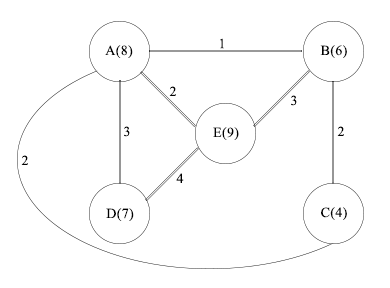
\includegraphics[scale=0.7]{ejercicio-4-ejemplo-entrada.png}
    \caption{Grafo de entrada}
    \label{fig:ej4_ejemplo}
\end{figure}

Contamos con la siguiente solución inicial (entre parentesis el peso de cada nodo):
\begin{center}
  \begin{tabular}{ l | c | r }
    $S_{1}$ & $S_{2}$ & $S_{3}$ \\ \hline
    A(3) & E(0) & D(0) \\
    B(4) &  &  \\
    C(3) &  &  \\
  \end{tabular}
  \textbf{Costo total:} 5
\end{center}

\begin{minipage}[t]{0.5\linewidth}
    \center{\textbf{(A)}} \\
    \raggedright{
        \textit{Tomo A:}\\
        $\rightarrow$ Lo pruebo en $S_{2}$: A(2) \checkmark Mejora
    }\\
    \begin{center}
      \begin{tabular}{ l | c | r }
        $S_{1}$ & $S_{2}$ & $S_{3}$ \\ \hline
        B(2) & E(2) & D(0) \\
        C(2) & A(2) &  \\
      \end{tabular}
      \textbf{Costo total:} 4
    \end{center}

    \raggedright{
        \textit{Tomo B:}\\
        $\rightarrow$ Lo pruebo en $S_{2}$: B(4) No mejora\\
        $\rightarrow$ Lo pruebo en $S_{3}$: B(0) \checkmark Mejora
    }\\
    \begin{center}
      \begin{tabular}{ l | c | r }
        $S_{1}$ & $S_{2}$ & $S_{3}$ \\ \hline
        C(0) & E(2) & D(0) \\
         & A(2) & B(0) \\
      \end{tabular}
      \textbf{Costo total:} 2
    \end{center}

    \raggedright{
        \textit{Tomo C:}\\
        $\rightarrow$ Lo pruebo en todos pero no mejora en ninguno por que tiene peso 0.
    }\\

    \raggedright{
        \textit{Tomo D:}\\
        $\rightarrow$ Lo pruebo en todos pero no mejora en ninguno por que tiene peso 0.
    }\\

    \raggedright{
        \textit{Tomo E:}\\
        $\rightarrow$ Lo pruebo en $S_{1}$: E(0) \checkmark Mejora
    }\\
    \begin{center}
      \begin{tabular}{ l | c | r }
        $S_{1}$ & $S_{2}$ & $S_{3}$ \\ \hline
        C(0) & A(0) & D(0) \\
        E(0) &  & B(0) \\
      \end{tabular}
      \textbf{Costo total:} 0
    \end{center}

    Hace una iteración mas buscando mejora pero no la encuentra, entonces termina. 

\end{minipage}
\vrule
\begin{minipage}[t]{0.5\linewidth}
    \centering{\textbf{(B)}}\\
    \raggedright{
        \textit{Tomo A y B:}\\
        $\rightarrow$ estan en el mismo subconjunto (no hago nada).
    }\\
    \raggedright{
        \textit{Tomo A y C:}\\
        $\rightarrow$ estan en el mismo subconjunto.
    }\\
    \raggedright{
        \textit{Tomo A y D:}\\
        $\rightarrow$ como peso(A en $S_{3}$ sin D)$+$peso(D en $S_{1}$ sin A) $<$ peso(A actual)+peso(D actual)
    }\\
    \begin{center}
      \begin{tabular}{ l | c | r }
        $S_{1}$ & $S_{2}$ & $S_{3}$ \\ \hline
        B(2) & E(0) & A(0) \\
        C(2) &  &  \\
        D(0) &  &  \\
      \end{tabular}
      \textbf{Costo total:} 2
    \end{center}
    \raggedright{
        \textit{Tomo B y A:}\\
        $\rightarrow$ no mejora.
    }\\
    \raggedright{
        \textit{Tomo B y C:}\\
        $\rightarrow$ estan en el mismo subconjunto.
    }\\
    \raggedright{
        \textit{Tomo B y D:}\\
        $\rightarrow$ estan en el mismo subconjunto.
    }\\
    \raggedright{
        \textit{Tomo B y E:}\\
        $\rightarrow$ no mejora.
    }\\
    \raggedright{
        \textit{Tomo C y A:}\\
        $\rightarrow$ no mejora.
    }\\
    \raggedright{
        \textit{Tomo C y B:}\\
        $\rightarrow$ estan en el mismo subconjunto.
    }\\
    \raggedright{
        \textit{Tomo C y D:}\\
        $\rightarrow$ estan en el mismo subconjunto.
    }\\
    \centering{...}\\
    No mejora en ninguna de las combinaciones siguientes.
    Termina.


\end{minipage}


\subsection{Análisis de complejidad temporal}
Sea $n$ la cantidad de vértices del grafo de entrada, y $k$ el parámetro de k-PMP. Vamos a usar el pseudocódigo ya introducido para el cálculo de complejidad de ambos algoritmos. Hay que mencionar que ésta se calcula para el peor caso de una iteración del ciclo más exterior de los algoritmos (\textit{while(hayMejora)}) ya que no podemos determinar cuantas veces se itera sobre este mismo. Lo que si se afirma es que termina cuando encuentra un óptimo local, es decir ninguno de sus vecinos tiene una mejor solución. Se omite la complejidad de la obtención de la solución inicial y se asume como entrada.
\\

\textbf{(A):}

\begin{itemize}
    \item Linea $5$: seteamos la variable \textit{hayMejora} en $O(1)$
    \item Linea $6$: iniciamos un ciclo que se repite n veces.
    \begin{itemize}
        \item Lineas $7$ y $8$: seteamos variables en $O(1)$ y calculamos el peso del nodo en cuestión en el subconjunto esto cuesta $O(n)$ (NO EXPLICITO EN EL PSEUDOCODIGO, esto lo hacemos para no calcularlo dentro del siguiente ciclo ya que aumentaria la complejidad.)
        \item Linea $9$: Se inicia otro ciclo sobre los subconjuntos que como peor caso se prueba cambiar el nodo a todos los subconjuntos y recorremos los $k$.
        \begin{itemize}
            \item Linea $10$: Checkeo booleano del if en $O(1)$
            \item Lineas $11$, $12$, $13$ y $14$: borrar e insertar nodos de un conjunto cuesta $O(\log n)$ y las asignaciones de variables $O(1)$. 

            Entonces tenemos $2O(\log n) + 2O(1)$

            Cómo peor caso esto ocurre una vez en las $k$ iteraciones ya que hace que salgamos de él.
            \item Linea $16$: aumentamos una variable en $O(1)$
        \end{itemize}
    \end{itemize}
\end{itemize}
Entonces tenemos:
\begin{center}
    $Complejidad(A) = O(1) + n(O(1)+O(n)+O(k)+2O(\log n)+2O(1)+O(1))$

    $Complejidad(A) = n(max\{O(n),O(k),O(\log n)\})$

    $Complejidad(A) = max\{O(n^2),O(nk),O(n\log n)\}$

    $Complejidad(A) = O(n^2)$
\end{center}

\textbf{(B):}

\begin{itemize}
    \item Linea $5$: seteamos la variable \textit{hayMejora} en $O(1)$
    \item Linea $6$: iniciamos un ciclo que se repite n veces.
    \begin{itemize}
        \item Lineas $7$ y $8$: seteamos variables en $O(1)$ y calculamos los pesos de ambos nodos en los dos subconjuntos, esto cuesta $4O(n)$ (esto lo hacemos para no calcularlos dentro del siguiente ciclo.)
        \item Linea $9$: Se inicia otro ciclo sobre los nodos (para checkear con quien swappeo) en peor caso se repita $n$ veces.
        \begin{itemize}
            \item Linea $10$: Checkea booleano del if en $O(1)$
            \item Lineas $11$ y $12$: Calcula el valor del peso del nodo en un subconjunto, como peor caso esto toma $O(n)$
            \item Linea $13$: Checkea booleano del if en $O(1)$
            \item Lineas $14$ a $19$: Borra e inserta nodos de un subconjunto a otro, cuesta $O(\log n)$ y las asignaciones de variables $O(1)$. 

            Entonces tenemos $4O(\log n) + 2O(1)$

            Cómo peor caso esto ocurre una vez en las $n$ iteraciones ya que hace que salgamos de él.
            \item Linea $16$: aumentamos una variable en $O(1)$
        \end{itemize}
    \end{itemize}
\end{itemize}

Entonces tenemos:
\begin{center}
    $Complejidad(B) = O(1) + n(O(1)+4O(n)+O(n)+4O(\log n)+2O(1)+O(1))$

    $Complejidad(B) = n(max\{O(n),O(\log n)\})$

    $Complejidad(B) = max\{O(n^2),O(n\log n)\}$

    $Complejidad(B) = O(n^2)$
\end{center}

\subsection{Test de complejidad}

Construimos 100 instancias aleatorias de grafos de $n$ vértices, para cada $n = {1, ... , 100}$. Para cada instancia, se calculó el tiempo de ejecución de la heurística con parámetro $k = {10, 20, ..., 100}$ cinco veces (tomando el mínimo), para luego calcular el promedio para cada $n$ separando por $k$. Así, para cada $n$ tenemos el tiempo de ejecución promedio de cada $k$. Como esperamos que la complejidad temporal sea $O(n^2)$ se dividió la muestra por $n$, esperando ver una recta, que es lo que efectivamente ocurre. Veamos el gráfico de los resultados del test:

%\begin{figure}[H]
%    \begin{minipage}[t]{\linewidth}
%		\centering
%		\frame{\includegraphics[width=\textwidth]{ejercicio-3-%complejidad-dividida-n.jpg}}
%		\label{fig:ejercicio_3_complejidad_dividida_n}
%    \end{minipage}
%\end{figure}
%
%Podemos observar que para cada $n \leq k$, el tiempo dividido por $n$ es una constante, lo cual tiene sentido porque habíamos acotado por $O(k)$ construir la solución trivial, y $O(n) \subseteq O(k)$ porque $n \leq k$. Recién a partir de $n = k+1$ el tiempo dividido $n$ se vuelve apreciable, y como esperábamos es una recta, lo que indica que es $O(n^2)$ como era nuestra hipótesis.

